\begingroup
\RaggedRight

\begin{quote}
``Security wins many battles but loses the security war. We are definitely going backwards in computer security.''
\newline
\hfill  — \textit{Adi Shamir, A.M. Turing Award Laureate}
\end{quote}


Hardware Trojan (HT) insertion involves a malicious alteration to a hardware component's design, posing risks such as device malfunction, data leakage, or physical damage \cite{francq2015introduction}. With the semiconductor industry adopting a fabless model, the potential for HT insertion at various manufacturing stages grows, posing a substantial security threat. Traditional detection methods, like signature-based approaches \cite{gbade2014signature}, prove ineffective against evolving HT attacks, prompting a shift towards Machine Learning (ML) solutions. However, existing ML approaches often lack information on datasets, struggle with concept drift, and require additional evaluation metrics \cite{285613}. A study in \cite{quiring2022and} questions the universality of ML in addressing hardware security concerns \cite{liu2021two}.

ML methods face challenges due to concept drift caused by intelligent modifications to HT insertion techniques. The thesis introduces \textbf{PALETTE}, an algorithm-agnostic framework for evolving hardware Trojan detection, utilizing conformal prediction \cite{shafer2008tutorial}. It provides risk-aware theoretical guaranteed coverage under covariate shift \cite{tibshirani2019conformal}. Non-invasive and applicable as a wrapper over existing ML models, \textbf{PALETTE} offers set predictions, ensuring the correct class is included 95\% of the time on average (i.e., $\alpha$ = 0.05).

HT insertion is a concern in fabless semiconductor manufacturing, with potential attacks at different stages \cite{salmani2017hardware, Regazzoni:HTDetection, Guin:HTDetection, Salmani:HTDetection}. Vulnerabilities span design phases, EDA processes, and post-production stages, necessitating robust security measures \cite{narasimhan2011tesr, muralidhar2021contrastive, chang2023supplier, panduro2023effective, monjur2023hardware}. Comprehensive approaches, while crucial, come with drawbacks, leading to the relevance of ML in countering HTs. Challenges like resource-intensive training, adversarial attacks, and interpretability are acknowledged.

Machine Learning has emerged as a potent tool for HT detection in fabless semiconductor manufacturing \cite{gubbi2023hardware, huang2020survey, liakos2019machine, koblah2023survey, koylu2023survey}. Challenges include acquiring diverse datasets, susceptibility to adversarial attacks \cite{west2023towards}, and the need for interpretability and explainability \cite{li2022interpretable, caruana2020intelligible}. \textbf{NOODLE}, proposed in this thesis, is an uncertainty-aware hardware Trojan detection using multimodal deep learning with graph representation and tabular data, performing binary classification.

\section*{Research Gap}

The shared identification of these gaps in research sets the stage for a thorough exploration plan, underscoring the particular areas that demand deeper investigation and focused development in the field of multimodal learning for detecting hardware trojans. A few of them are discussed below:

\begin{itemize}

    \item \textbf{Dataset Transparency and Class Distribution} - The lack of transparency in revealing comprehensive dataset details, especially concerning class distribution differences, highlights a research gap. There is a need for scholarly attention to address transparency issues and gain a nuanced understanding of dataset characteristics in the presence of significant class distribution variations.
    
    \item \textbf{Concept Drift in Model Evaluation} - The insufficiency in considering "concept drift" stemming from adversaries' evolving insertion techniques introduces a research gap. Coping strategies are required to effectively handle concept drift, indicating the necessity for further exploration and validation in this area.
    
    \item \textbf{Custom metrics for Model Evaluation} - The inadequacy of conventional metrics for model evaluation underscores a research gap. There is a need for additional measures to strengthen traditional evaluation methods, ensuring reliable decision-making and comprehensive prediction coverage.
    
    
    \item \textbf{Uncertainty-Aware Multimodal Learning} - The limited exploration of diverse multimodal approaches, particularly beyond prevalent graph representation and tabular data, is identified as a research gap. Scholarly inquiry and investigation into various modality combinations in multimodal learning for hardware trojan detection are needed.
    

    
    \item \textbf{Interpretability and Explainability} - The acknowledgment of the significance of interpretability and explainability in multimodal models highlights a research gap. The development of interpretable multimodal hardware trojan detection models is necessary to enhance trust and understanding in the domain.

\end{itemize}


\iffalse
\begin{figure}
  \centering
   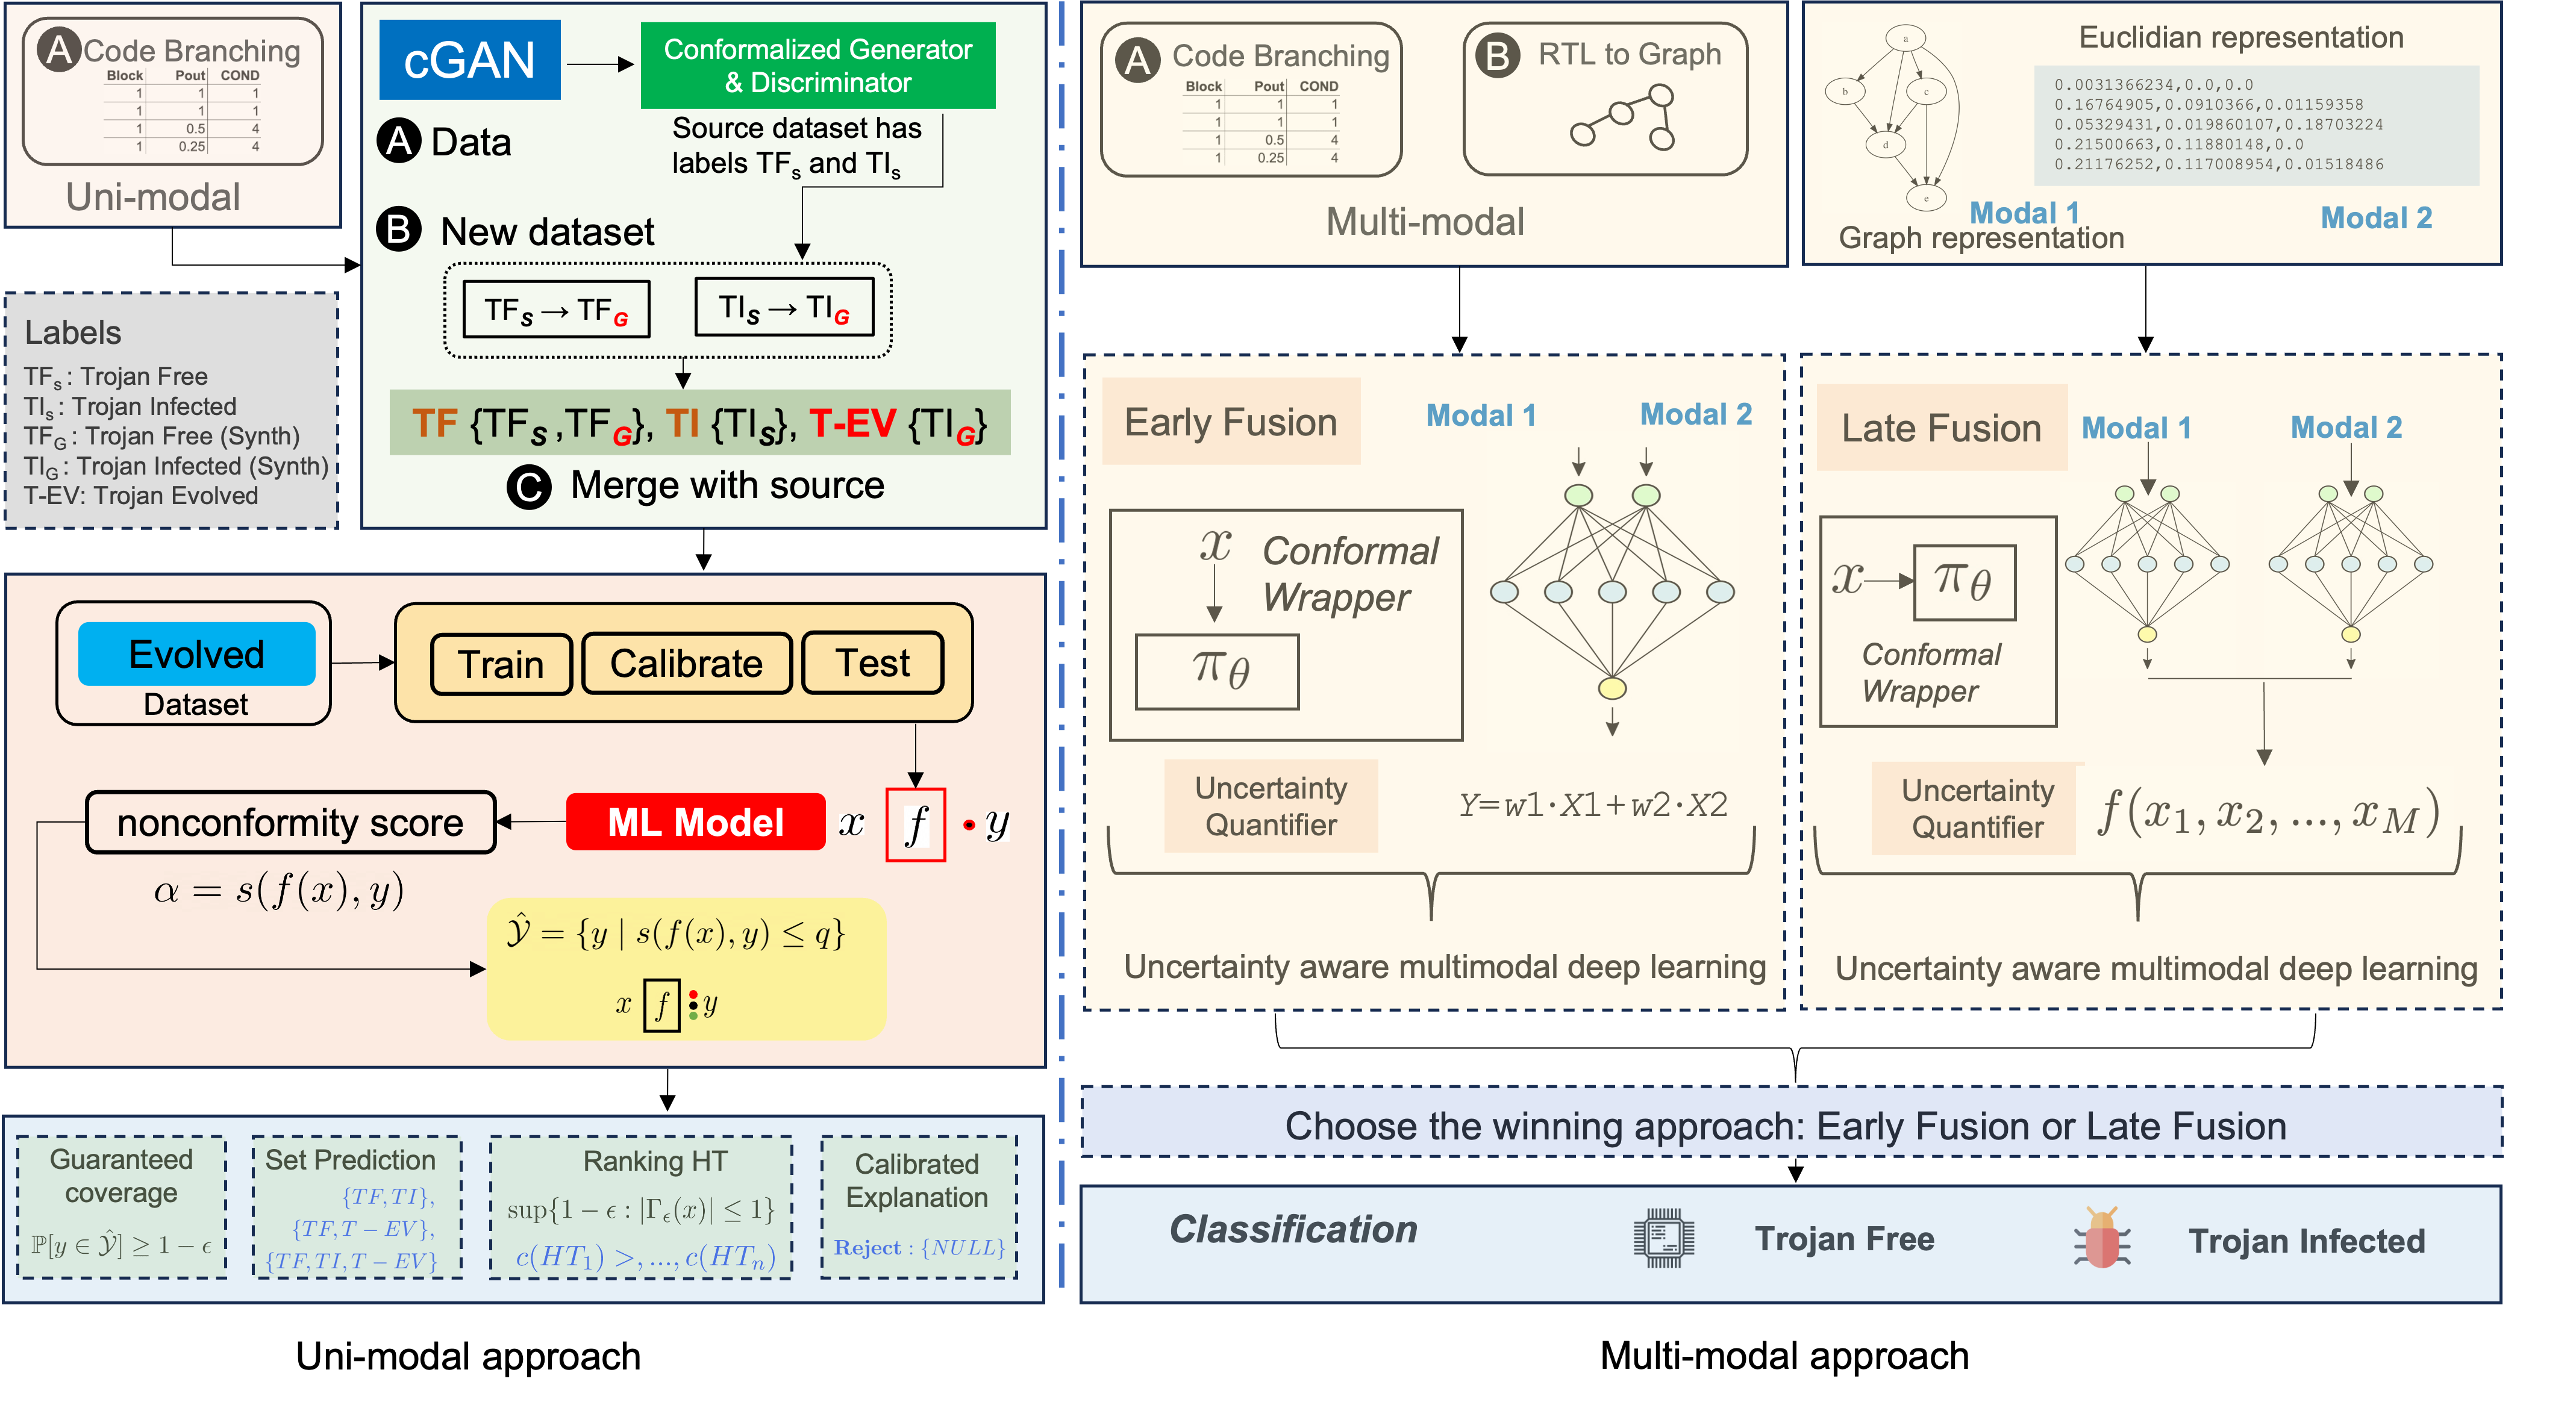
\includegraphics[width=1\linewidth]{figs/solution_thesis.png}
   \caption{The input feature is passed to a conventional machine learning hardware Trojan detector. This detector produces a result and is compared to conformal inference, which provides an uncertainty measure and a confidence set for each detected evolved hardware Trojan.}
  \label{fig:introduction}
\end{figure}
\fi 



\section*{Preliminaries}
\label{Sec:Prelem}
%Background 

%%%%%%%%%%%%%%%%%%%%%%%%%%%%%%%%%%%%%%%%%%%%%%%%%%%%%
    %Calibration
%%%%%%%%%%%%%%%%%%%%%%%%%%%%%%%%%%%%%%%%%%%%%%%%%%%%%
\subsection*{Calibrated Prediction}
\label{sec:Calibration}
Calibration involves ensuring that a model's confidence score accurately reflects the true probability of the prediction's correctness \cite{ovadia2019can}. Let $X$ be the input data, and $Y$ be the output label. Given a training dataset $D = {(x_1, y_1), (x_2, y_2),..., (x_n, y_n)}$, the goal is to learn a function $f$ that can predict the correct output label $y$ for a given input $x$. The output of the model for an input $x$ can be denoted as $f(x)$, and the true probability of the prediction's correctness can be denoted as $P(y=1|x)$. A calibrated model produces a confidence score $g(x)$ that reflects the true probability of correctness of the prediction. The goal of calibration is to ensure that the confidence score $g(x)$ is well-calibrated, i.e., $P(y=1|g(x)=p) = p$ for all $p$ in the range $[0, 1]$.

\textbf{Why we need calibration?}

Calibration is a crucial aspect in HT detection since it aids in determining the likelihood of the existence of a Trojan in a circuit, which can have a significant impact on decision-making. In situations where a model's confidence score is high, but the likelihood of a Trojan's presence is low, it is reasonable to assume that the circuit does not contain a Trojan. Conversely, if the confidence score is low but the likelihood of a Trojan's presence is high, further investigation of the circuit is necessary.

%%%%%%%%%%%%%%%%%%%%%%%%%%%%%%%%%%%%%%%%%%%%%%%%%%%%%
    %Conformal Prediction
%%%%%%%%%%%%%%%%%%%%%%%%%%%%%%%%%%%%%%%%%%%%%%%%%%%%%
\subsection*{Conformal Prediction}
\label{sec:CP}
%Conformal prediction is a framework for constructing prediction intervals that are guaranteed to have a specified level of coverage probability, typically at a confidence level of $1-\alpha$ for some pre-specified $\alpha \in (0,1)$. Given a training set ${(X_test, y_test)}{i=1}^n$, where $x_i \in \mathcal{X}$ is a feature vector and $y_i \in \mathcal{Y}$ is a label, the goal is to construct a function $f: \mathcal{X} \rightarrow \mathcal{Y}$ that predicts the label $y$ for a given feature vector $x$. Conformal prediction produces prediction sets $\Gamma(x)$ for a new feature vector $x$ such that $P(y \in \Gamma(x) | x, {(x_i, y_i)}{i=1}^n) \geq 1 - \alpha$ for all $x \in \mathcal{X}$ and for all $y \in \mathcal{Y}$, where $P$ is the probability measure. The prediction sets can be constructed using various methods, including the nonconformist algorithm and the transductive conformal prediction algorithm.

Conformal prediction \cite{shafer2008tutorial} is a ML framework that quantifies prediction uncertainty by generating prediction sets. It enhances the inference of traditional models, ensuring reliable validity and enabling confidence estimation for individual predictions. In the context of detecting HTs, label-conditional validity is a vital property when dealing with an imbalanced dataset where label proportions differ significantly. This is particularly relevant since the likelihood of encountering a Trojan on a circuit is generally low. In addition, it is worth noting that minority classes are often disproportionately impacted by errors when label-conditional validity is absent \cite{lofstrom2015bias}. However, this issue can be mitigated by ensuring label-conditional validity, which guarantees that the error rate for even the minority class will eventually converge to the chosen significance level in the long term. Sometimes, conformal prediction may produce uncertain predictions, meaning that prediction sets contain more than one value. This occurs when none of the labels can be rejected at the specified significance level.

When using conformal prediction, the confusion matrix differs slightly from the conventional one due to the unique nature of \textit{prediction sets}, which consist of multiple values rather than a single value. In the case of binary classification, it is essential to consider the number of correctly predicted examples, which have a prediction set containing only the correct label, as well as the number of incorrectly predicted examples, where the prediction set includes only the incorrect label. Additionally, it is important to take into account the number of inconclusive predictions that occur when the prediction set contains both labels, as well as the number of examples with an \textit{empty prediction set}. Furthermore, in some cases, it may be more appropriate to provide a \textit{single value point prediction} instead of a prediction set or interval in a hedged forecast. In such cases, selecting the label with the highest $p$-value is a simple and reasonable option. The point prediction can be hedged by incorporating additional information that describes the uncertainty.


\begin{figure*}[ht]
  \centering
   
\includegraphics[width=0.95\linewidth]{figs/frameowrk_cp.png}
   \caption{Illustration of Conformal Prediction Framework, showcasing the key components and stages involved in the process.}
  \label{fig:frameowrk_cp}
\end{figure*}


In this thesis our work relies on Mondrian Inductive Conformal Prediction (ICP) \cite{bostrom2021mondrian} as shown in Algorithm \ref{algo:mcp}. Furthermore, to decrease the rate of false negatives in alert systems, we require class-based authenticity for samples classified as "Evolving Trojan". Additionally, we must ensure that the samples labeled as "Evolving Trojan" are indeed genuine to attain this goal.

\begin{algorithm}[t]
\SetKwInOut{Input}{Input}
\SetKwInOut{Output}{Output}
\Input{Training data $D$, test instance $x$, significance level $\alpha$, number of trees $T$, and maximum tree depth $d$.}
\Output{Prediction set $C(x)$ for $x$.}
Divide $D$ into $T$ disjoint subsets $D_1, \ldots, D_T$;

\For{$t \leftarrow 1$ \KwTo $T$}{
Sample $D_t'$ from $D_t$ by recursively partitioning $D_t$ along randomly chosen hyperplanes until each partition contains at most $2d$ points.

Train a classification model $M_t$ on $D_t'$.
}
Compute the conformity scores $s_t(x)$ of $x$ with respect to each model $M_t$.

Sort the conformity scores $s_t(x)$ in decreasing order.

Compute the $p$-values $p_t$ of the $T$ conformity scores $s_t(x)$ using the formula $p_t = \frac{T - t + 1}{T}$.

Compute the threshold $h$ such that $h = s_t(x)$ if $p_t > \alpha$, otherwise $h = \infty$.

Construct the prediction set $C(x)$ as the set of all labels $y$ such that $s_t(y) \geq h$ for all models $M_t$.

\Return $C(x)$
\caption{Mondrian ICP}
\label{algo:mcp}
\end{algorithm}

When calculating the non-conformity scores, we only consider the scores related to the examples that share the same class as the object $x_{n+1}$, which we are testing hypothetically as shown below: 
$$
p_{n+1}^{C_k}=\frac{\left|\left\{i \in 1, \ldots, q: y_i=C_k, \alpha_{n+1}^{C_k} \leq \alpha_i\right\}\right|}{\left|\left\{i \in 1, \ldots, q: y_i=C_k\right\}\right|}
$$


%%%%%%%%%%%%%%%%%%%%%%%%%%%%%%%%%%%%%%%%%%%%%%%%%%%%%
    %Coverage guarantee
%%%%%%%%%%%%%%%%%%%%%%%%%%%%%%%%%%%%%%%%%%%%%%%%%%%%%
\subsection*{Guaranteed Coverage of Prediction}
\label{sec:Coverage}
In the domain of HT detection, it is not only important to have a high level of confidence in the predictions made by a model but also a guarantee of the coverage of each prediction. The property of guaranteed coverage is an inherent property of conformal prediction, which provides statistical guarantees of the correctness of the model's predictions \cite{angelopoulos2023conformal}. The theoretical guarantee of coverage is based on the significance level, which is the probability of the model making a mistake. For example, if we set the significance level to $0.05$, it means that we allow the model to make mistakes $5\%$ of the time.

%Let $X$ be the input data and $Y$ be the output label. Given a training dataset $D = {(x_1, y_1), (x_2, y_2),..., (x_n, y_n)}$, the goal is to learn a function $f$ that can predict the correct output label $y$ for a given input $x$.
%The conformal prediction algorithm works by constructing a prediction set for each input $x$ in the test dataset. This prediction set is a set of potential output labels that the model predicts with a high degree of confidence. The size of the prediction set depends on the significance level and the quality of the model. Let $C(x)$ be the prediction set for the input $x$. We provide a mathematical proof of the guaranteed coverage of predictions by conformal prediction. 
The theoretical guarantee of coverage is valid for any input $x$, that the true output label $y$ will be contained in the prediction set $C(x)$ with a probability of at least $1 - \alpha$, where $\alpha$ is the significance level. Mathematically, this can be expressed as:

$$
P(y \in C(x)) \geq 1 - \alpha
$$

In other words, the probability of making a mistake is bounded by $\alpha$, and as $\alpha$ decreases, the size of the prediction set decreases, leading to higher confidence in the model's predictions. Similarly, if the value of $\alpha$ increases, consequently the size of the prediction set also increases; however, this also reduces the significance level (confidence) of the predictions. 

For example, if we set $\alpha = 0.05$, it means that we are $95\%$ confident that the true output label $y$ is contained in the prediction set $C(x)$ for any input $x$. The use of conformal prediction provides a strong theoretical guarantee of the correctness of the model's predictions in the context of HT detection, and the corresponding proof is given in Theorem \ref{thm:coverage}.

\begin{theorem}\label{thm:coverage}
Let $\mathcal{D}$ be a probability distribution over a set $\mathcal{X} \times \{0,1\}$, where $\mathcal{X}$ is a set of input features and $\{0,1\}$ is the set of labels. Let $f: \mathcal{X} \to \{0,1\}$ be a binary classifier, and let $\epsilon \in (0,1)$ be a confidence level. Then, the conformal prediction algorithm outputs a set of predictions $C(x) \subseteq \{0,1\}$ for each input $x \in \mathcal{X}$ such that:

\begin{equation*}
\mathbb{P}[(x,y) \sim \mathcal{D}, y \in C(x)] \geq 1-\epsilon
\end{equation*}

where $(x,y) \sim \mathcal{D}$ denotes sampling a pair $(x,y)$ from the distribution $\mathcal{D}$.

\end{theorem}

\begin{proof}
The proof follows from the construction of the conformal prediction algorithm. Given an input $x$, the algorithm outputs a set of predictions $C(x)$ based on the observed labels of the training examples with similar input features to $x$. The algorithm guarantees that each prediction in $C(x)$ has a $p$-value less than or equal to $\epsilon$ for any new input with the same feature vector as $x$. Since the algorithm outputs a set of predictions, the probability that at least one of the predictions is correct is at least $1-\epsilon$. 
\end{proof}

\begin{corollary}\label{cor:coverage}
Let $\mathcal{D}$, $f$, and $\epsilon$ be as in Theorem~\ref{thm:coverage}. For any sample size $n$, the conformal prediction algorithm outputs a set of predictions $C(x_1),\ldots,C(x_n)$ for each input $x_1,\ldots,x_n \in \mathcal{X}$ such that:

\begin{equation*}
\mathbb{P}[\forall i \in \{1,\ldots,n\}, (x_i,y_i) \sim \mathcal{D}, y_i \in C(x_i)] \geq 1-\epsilon
\end{equation*}

where $(x_i,y_i) \sim \mathcal{D}$ denotes sampling a pair $(x_i,y_i)$ from the distribution $\mathcal{D}$ for each $i$.

\end{corollary}

\begin{proof}
The proof follows from a union bound over the $n$ samples:

\begin{equation*}
\begin{aligned}
&\mathbb{P}[\forall i \in \{1,\ldots,n\}, (x_i,y_i) \sim \mathcal{D}, y_i \in C(x_i)] \\
&\geq 1 - \sum_{i=1}^n \mathbb{P}[(x_i, y_i) \sim \mathcal{D}, y_i \notin C(x_i)] \\
&\geq 1 - n \epsilon
\end{aligned}
\end{equation*}

where the second inequality follows from Theorem~\ref{thm:coverage}. 
\end{proof}


\subsection*{Multimodal Learning}
\label{sec:multimodal}
Multimodal learning \cite{ngiam2011multimodal} addresses complex problems by integrating information from multiple modalities, such as text, images, and audio, to obtain a comprehensive understanding of a given phenomenon. In our case, we use graphical data and tabular representations of the source circuits. This approach enables models to capture nuanced relationships that may be overlooked when considering each modality in isolation, and thus empowers the model to make more robust predictions.

From a mathematical perspective, multimodal learning involves the integration of data representations into a unified framework. Let \(X_1, X_2, ..., X_M\) represent \(M\) different modalities of data, each with their respective feature spaces \(\mathcal{F}_1, \mathcal{F}_2, ..., \mathcal{F}_M\). The task is to learn a mapping \(f\) that captures the relationships between these modalities. Mathematically, this can be formulated as:
\begin{equation}
f: \mathcal{F}_1 \times \mathcal{F}_2 \times ... \times \mathcal{F}_M \rightarrow \mathcal{Y}
\end{equation}
where \(\mathcal{Y}\) is the target space, representing the desired prediction.

The challenge lies in effectively combining information from diverse modalities, which can be approached through various techniques such as late fusion or early fusion. 

In late fusion \cite{trong2020late}, features are extracted independently from each modality and then combined at a later stage. This approach treats modalities as separate entities until a decision needs to be made and can be represented as:
\begin{equation}
f(x_1, x_2, ..., x_M) = g(h_1(x_1), h_2(x_2), ..., h_M(x_M))
\end{equation}
where \(h_i\) represents feature extraction for modality \(i\), and \(g\) combines the extracted features.

In early fusion \cite{nguyen2021gefa}, information from different modalities is combined at the input level, resulting in a joint feature representation which can be expressed as:
\begin{equation}
f(x_1, x_2, ..., x_M) = h(x_1, x_2, ..., x_M)
\end{equation}
where \(h\) combines the raw input data from all modalities.

\section*{Related Works}
\label{Related}
HT detection using traditional ML techniques has primarily focused on modeling methods, and it involves developing and implementing algorithms that can improve overall accuracy in detecting HTs. The input to the model consists of the features extracted from the Register Transfer Level (RTL) code as tabular and graphical representations of the circuit. Different surveys on ML for detecting HT attacks have been conducted in \cite{huang2020survey}, \cite{gubbi2023hardware}, \cite{koylu2023survey}, and \cite{kundu2021application}. In \cite{botero2021hardware} and \cite{ashok2022hardware} image classification is used, and in \cite{10027082} multimodal image processing is utilized. Most of the papers have focused on feature extraction from gate-level netlists and using ML models such as Support Vector Machine (SVM) \cite{bao2014application}, Neural Network (NN) \cite{hasegawa2017hardware}, eXtreme Gradient Boosting (XGB) \cite{dong2019machine}, and Random Forest (RF) classifier \cite{hasegawa2017trojan}.

% RL
With the success of Reinforcement Learning (RL) in other domains, a few works have adapted RL in the hardware security domain, such as RL-based static detection \cite{gohil2022attrition}, and RL with adaptive sampling for on-chip detection \cite{chen2023adatest}. In these methods, a common approach involves training the classifier model initially and then adjusting the hyperparameters of the classifier. This adjustment process aims to minimize the false negative rate and, in turn, improve the model's accuracy. Graph Neural Network (GNN) \cite{alrahis2022embracing,hepp2022golden} and Abstract Syntax Tree (AST) \cite{han2019hardware} are generated for the RTL code; however, it is still not clear how the graphs can carry forward not only the structural but also the behavioral attributes of the circuit.

% Drift 
Furthermore, dealing with concept drift is crucial after deploying a model because the newly acquired data can be significantly dissimilar to the data the model was originally trained on. One such work in security applications is shown in \cite{yang2021cade} which involves the mapping of data samples into a space with fewer dimensions and the automatic learning of a distance function that can evaluate the differences between them. The concept drift, however, has not been studied in the HT domain even though HTs can evolve over time.

% Explainability 
The explainability aspect of ML is also covered in the hardware security domain; for example, \cite{pan2023hardware}, \cite{downing2021deepreflect}, and \cite{severi2021explanation} have used SHapley Additive exPlanations (SHAP) on benchmark datasets and have shown promising results. However, a drawback of utilizing SHAP is that it comes with inherent issues such as disregarding causality and being affected by human bias. It merely assesses the extent to which features contribute to a given dataset, without providing an explanation of how they would behave in the actual world, which may differ from the dataset used.

The emphasis in traditional ML approaches for HT detection has primarily been on modeling techniques. This entails the development and implementation of algorithms aimed at enhancing the overall accuracy of HT detection. The model takes as input features extracted from the Register Transfer Level (RTL) code, which are represented both in tabular and graphical forms depicting the circuit. Various surveys on the application of ML in detecting HT attacks have been conducted.  
Many research papers have concentrated on extracting features from Register Transfer Level (RTL) or gate-level netlists and employing ML models such as Support Vector Machine (SVM) \cite{bao2014application}, Neural Network (NN) \cite{hasegawa2017hardware}, eXtreme Gradient Boosting (XGB) \cite{dong2019machine}, and the Random Forest (RF) classifier \cite{hasegawa2017trojan}. In \cite{ashok2022hardware}, image classification techniques are also employed. %while in \cite{10027082}, a multimodal image processing approach is utilized, the only paper that detects HTs using multimodal image processing.

Multimodal Deep Learning (DL) has been a well-explored topic in the Artificial Intelligence (AI) community. Early research, exemplified by Deep Boltzmann Machines (DBM) focused on the model's capacity to understand probability distributions across inputs with multiple modes \cite{srivastava2012multimodal}. Additionally, applications of uncertainty-aware multimodal learning \cite{wang2022uncertaintyaware} have been successfully demonstrated in healthcare \cite{sarawgi2021uncertainty} and in scenarios involving multimodal task distributions \cite{almecija2022uncertaintyaware}, particularly in safety-critical environments. In our work, we target the fusion of graph \cite{ektefaie2023multimodal, kim2023heterogeneous} and Euclidean data as the modalities of interest along with uncertainty estimation. 

Moreover, when working in the hardware security domain, it is expected to have fewer data points that are malicious or Trojan-infected. In this context, it is necessary to work with small data \cite{nyiri2023can} and this has been achieved in various domains such as material science \cite{xu2023small} and anomaly detection \cite{ghamisi2023anomaly}.

\section*{Contributions}
\label{Contribution}
In this thesis, our primary focus revolves around multimodal deep learning for the identification of hardware trojans, and addressing the inherent challenges associated with this problem, for example, missing modalities and imbalanced dataset. The first challenge pertains to effectively handling missing modalities and implementing uncertainty-aware multimodal fusion approaches. To address this, we utilize graphical representations of circuits \cite{yu2021hw2vec} and Euclidean data derived from processing the Abstract Syntax Tree (AST) of RTL files (Verilog) \cite{px6s-sm21-22}. While multimodal approaches have been employed to enhance model accuracy in various domains, their application in Trojan identification has been notably absent. For uncertainty-aware multimodal learning, we advocate for implementing logic at the information fusion level of modalities, leveraging $p$-values aggregation with conformal prediction.

The second challenge we tackle is the quantification of uncertainty associated with hardware trojan prediction outcomes and ensuring the validity of predicted labels, especially when dealing with a limited number of highly imbalanced data points. Specifically, our interest lies in the ability of a machine learning classifier to predict the true label of a new data point with a 95\% provable guaranteed coverage, a crucial requirement in risk-sensitive domains. Designing such a system holds potential benefits for decision-makers investigating detected labels as "Trojan-Infected." Additionally, we explore the possibility of ranking detected "Trojan-Infected" circuits to enable more informed treatment decisions.

Our primary contributions are summarized as follows:

\begin{itemize}
\item Proposing a \textbf{multimodal learning approach using graph and euclidean data} of the hardware circuits. This study is the first to investigate and implement a multimodal approach for HT detection, emphasizing uncertainty-awareness.
\item Suggesting a \textbf{model fusion approach that leverages $p$-values as statistical measures}, systematically assessing each modality's contribution to the overall prediction. This enhances interpretability and facilitates more robust decision-making.
\item Addressing the \textbf{challenges of missing modalities} and solving the issue of handling an imbalanced and small dataset by leveraging generative adversarial networks. Introducing the notion of HT evolution and providing an innovative method of creating evolving HTs with high precision using a conformalized generative adversarial network.
\item Novel concept of \textbf{guaranteed coverage of the prediction set}, proposing a tunable significance level through conformal prediction for HT detection. Additionally, defining an algorithm-agnostic and explainability-aware reject prediction made by the ML model. When the model is uncertain about identifying the evolving Trojan, it rejects the prediction, passing it to a human for manual investigation.
\item Proposing a \textbf{ranking mechanism for the evolved Trojans} by assigning a confidence score from the prediction. This contribution is validated on synthetic and real chip-level HT-induced benchmarks.
\end{itemize}


\endgroup